\section*{Branching Ratio}

The first step to evaluate the branching ratio between o-Ps and p-Ps consisted in the selection of the correct decay channel by mean of detectors geometry and signals coincidence.
As above mentioned p-Ps decays with the emission of two collinear photons with the same energy, due to the fact that positronium annihilation occurs essentially at rest, while o-Ps, for the same reason, decays with the emission of three coplanar photons, with an emission angle between them dependent on their energy.

In order to select the p-Ps decay channel, an angle of 180$^\circ$ was imposed between two of the three detectors on the goniometer~(see Fig~\ref{Fig:PsGeometry}-\emph{a}), and their coincidence was used as trigger signal for the digitizer. 

The o-Ps decay channel was selected, instead, placing the three detectors at 120$^\circ$ between them~(see Fig~\ref{Fig:PsGeometry}-\emph{b}) and using the triple coincidence as trigger signal for the digitizer. A longer acquisition time with respect to the first configuration was necessary due to the lower counter rate.

 
\begin{figure}[h!]
	\centering
	\subfloat[][\emph{p-Ps geometry}.]
	{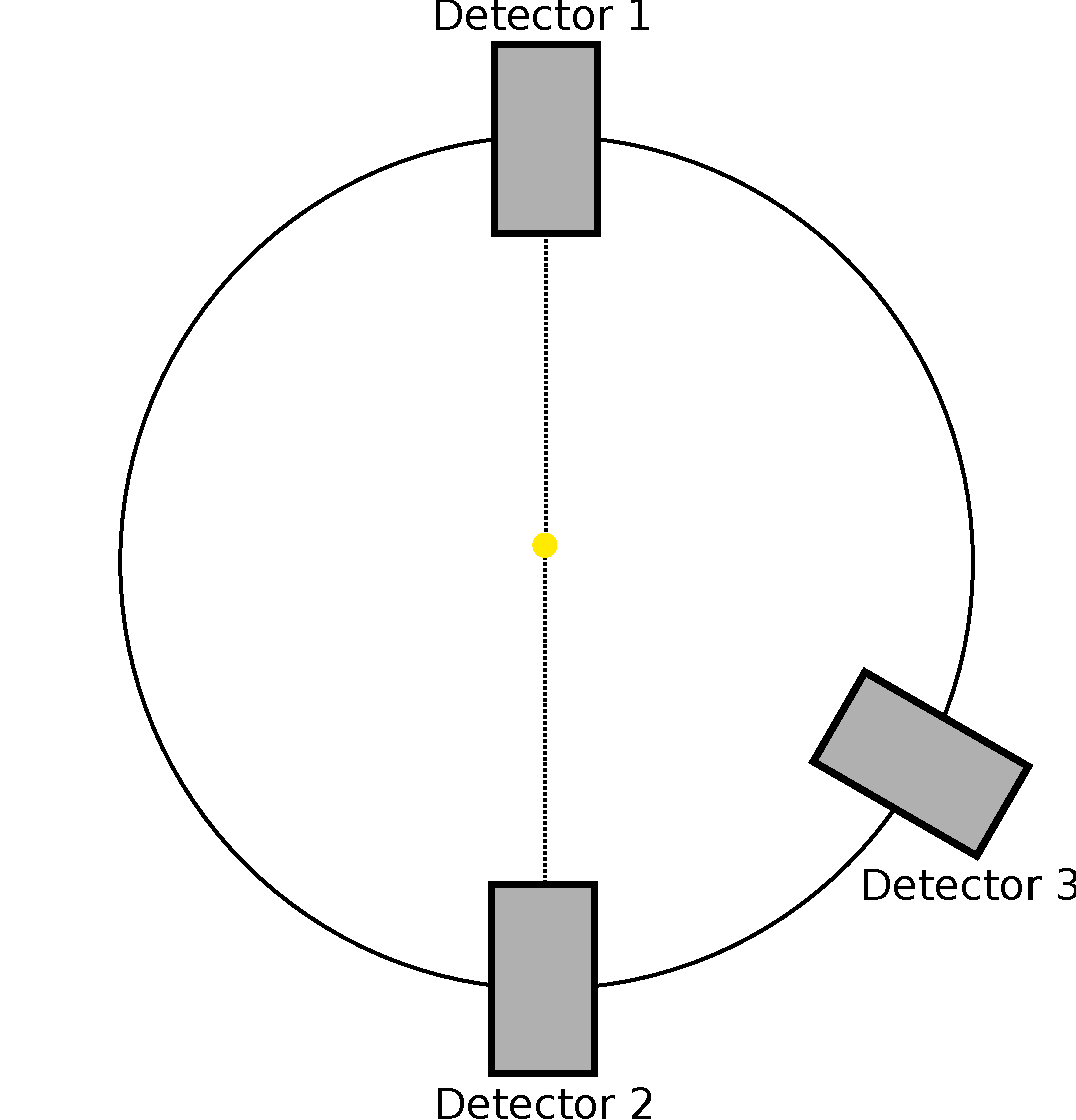
\includegraphics[width=.45\textwidth]{pPsGeometry}} \quad
		\subfloat[][\emph{o-Ps geometry}.]
	{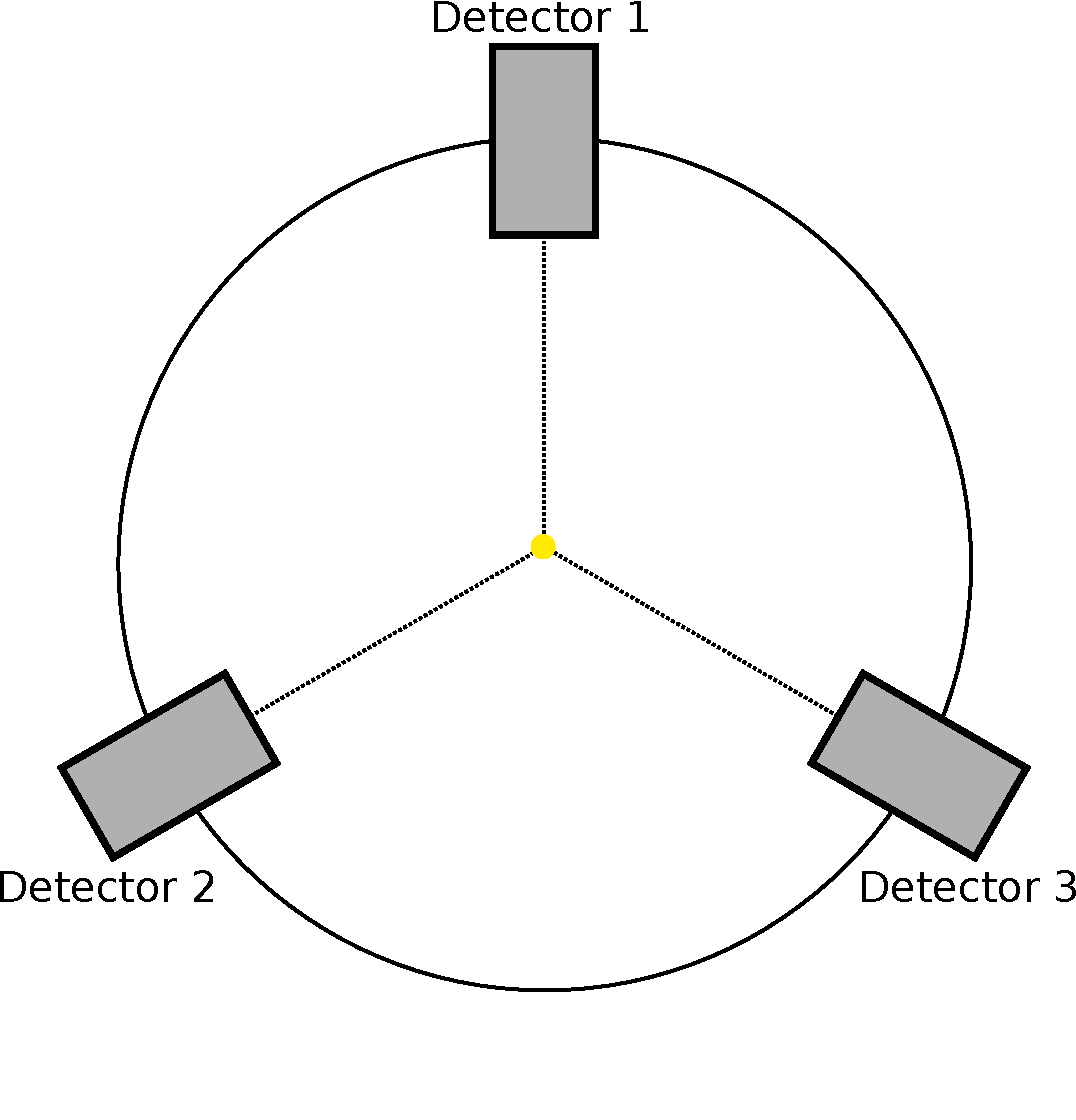
\includegraphics[width=.45\textwidth]{oPsGeometry}} \\
	\caption{Geometry of the experimental setup chosen for the p-Ps~(\emph{a}) and o-Ps~(\emph{b}) decay channel selection.}
	\label{Fig:PsGeometry}
\end{figure}

The spectra recorded by the two detectors for the p-Ps configuration are presented in Fig. \ref{Fig:pPs_spectra_bkg}.
\begin{figure}[H]
\centering
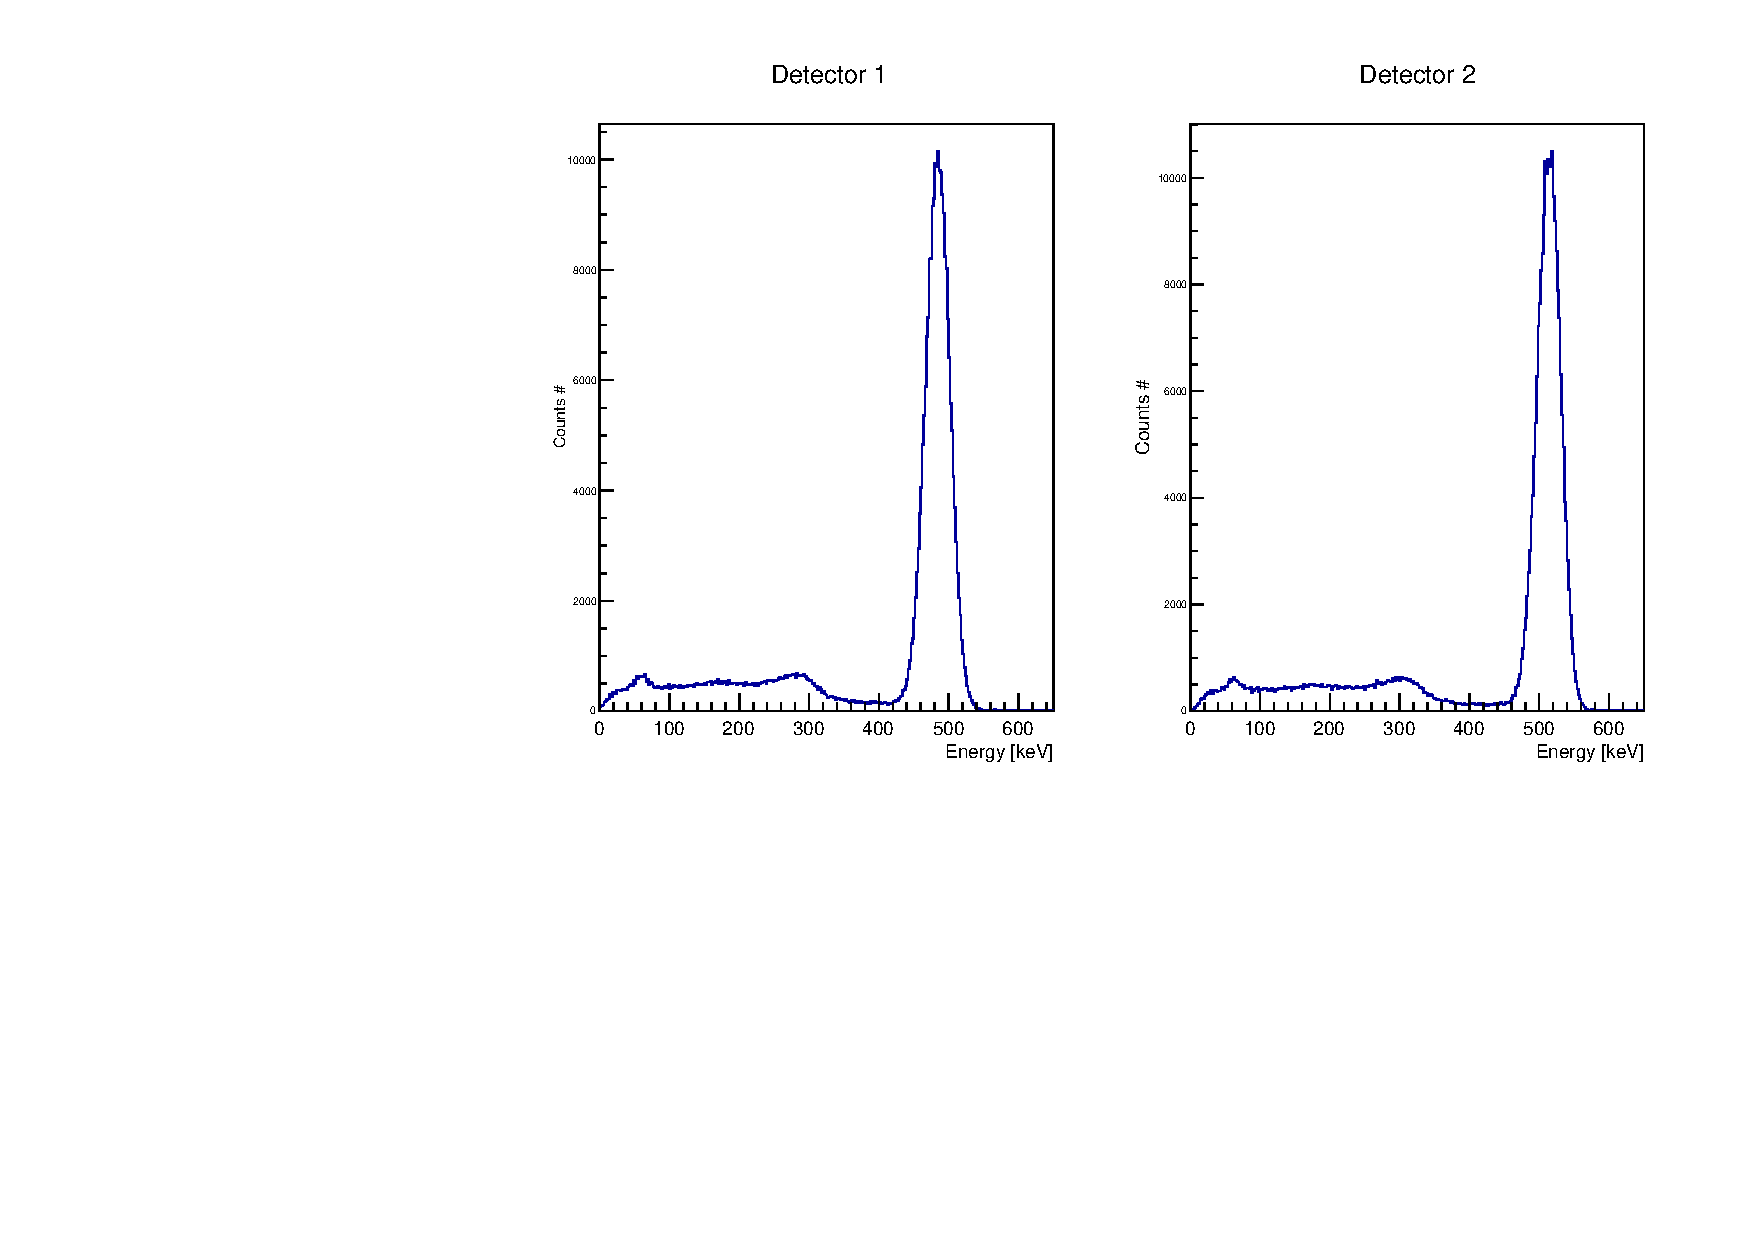
\includegraphics[width = 0.8\textwidth]{two_coinc_wbg}
\caption{2-$\gamma$ coincidence. From configuration 1}
\label{Fig:pPs_spectra_bkg}
\end{figure}

In order to determine the number of detected para-positronium decay events, the photopeak has to be integrated.
Before integrating the photopeak, however, the Compton Background has to be removed as in Fig \ref{Fig: removed compton back}.

\begin{figure}[H]
\centering
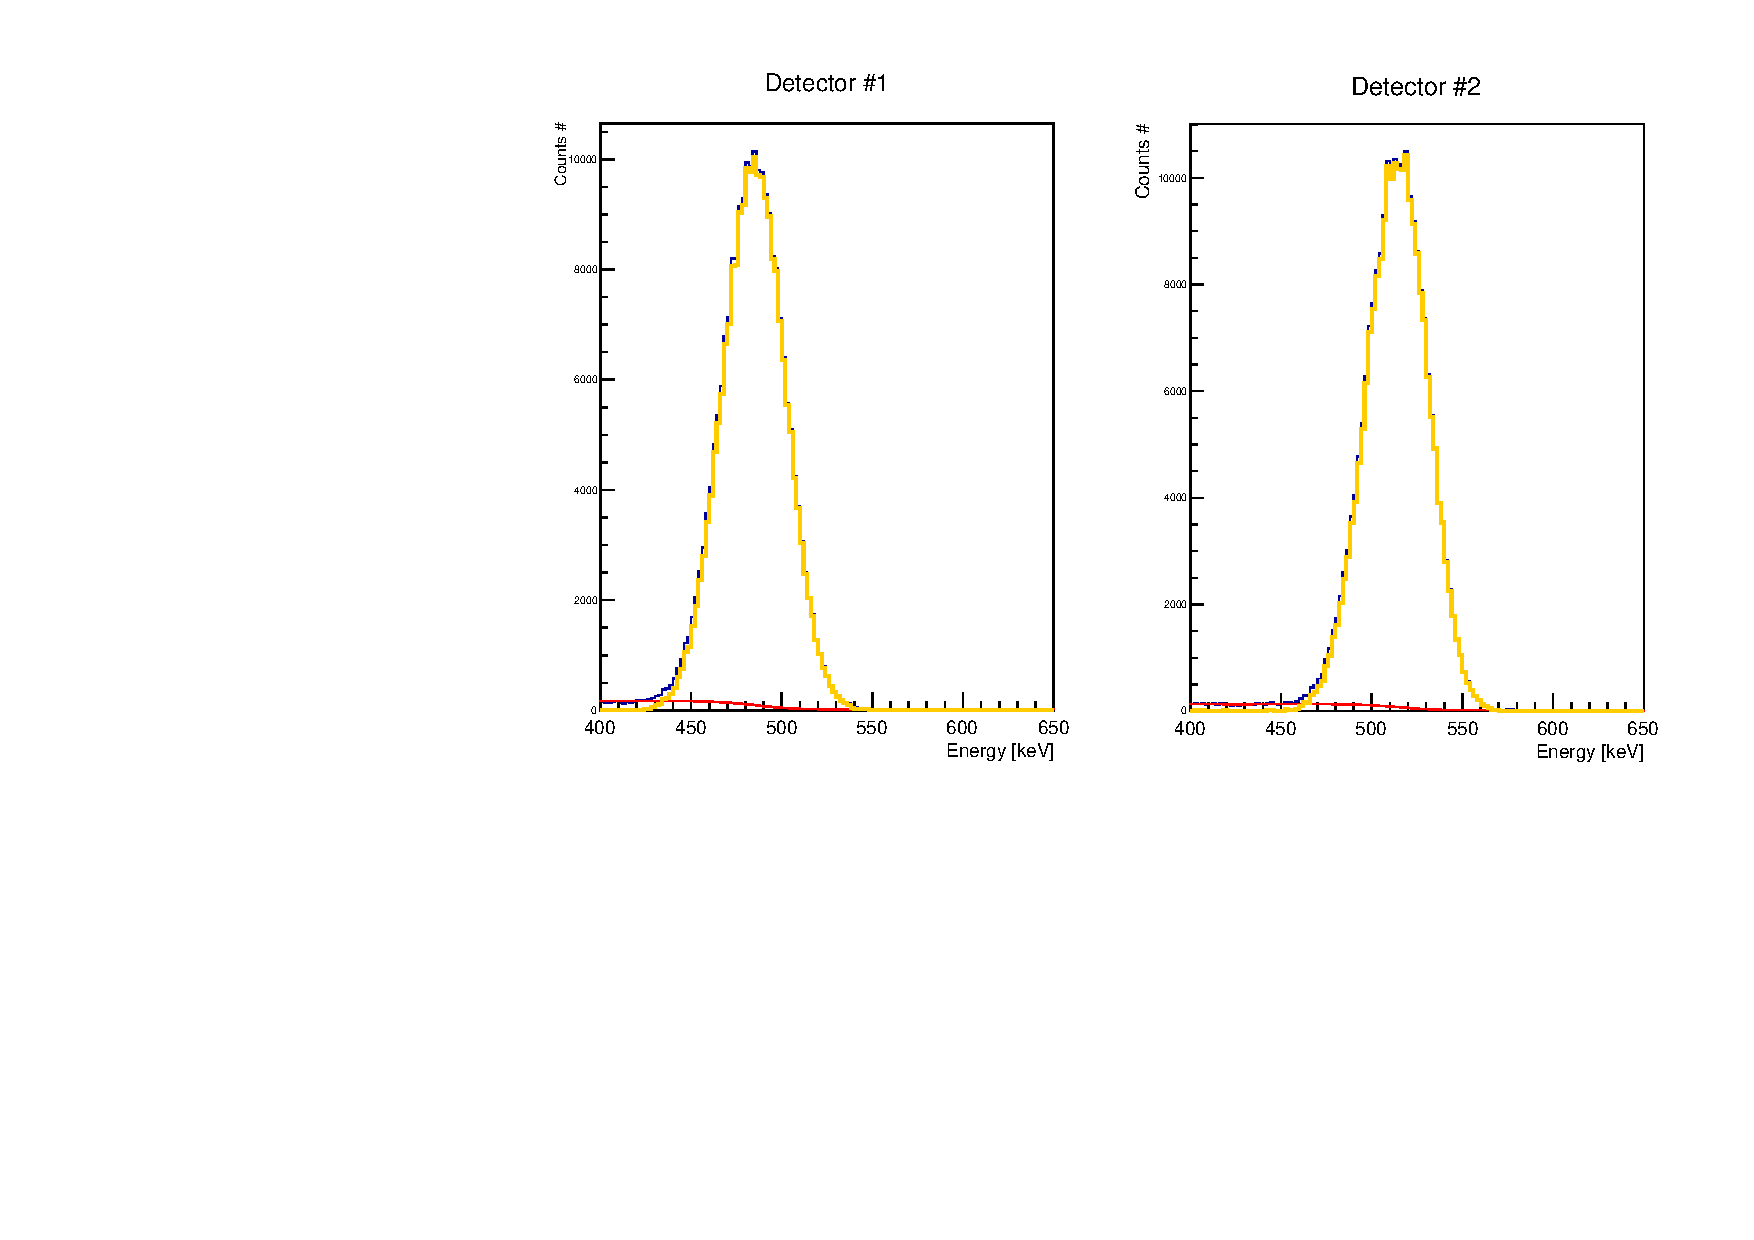
\includegraphics[width = 0.8\textwidth]{coinc_back}
\caption{2-$\gamma$ coincidence with removed background.}
\label{Fig: removed compton back}
\end{figure}

After that the photopeak could be integrated resulting in a yields of:
\begin{equation}
N_{2\gamma} = 218248
\end{equation} 

The number of obtained events has to be corrected due to the fact that not all para positronium decay events are detected and then counted. With the purpose of correcting this measure, we need an estimate of the covered solid angle in this configuration:
\begin{equation}
f_{2\gamma} = \dfrac{2\pi r^2}{4\pi d}
\end{equation}
that lead to an estimate for the number of parapositronium decay events of:
\begin{equation}
N_{2\gamma} = \dfrac{N_{2\gamma}^{\text{measured}}}{f_{2\gamma}}
\end{equation}




